\documentclass[color=pdftex,dvipsnames,usenames,svgnames,table]{guitbeamer}

\usepackage{xcolor}
\usepackage[color]{guit}
\usepackage{type1cm}
\usepackage{listings}
\usepackage{graphicx}
\usepackage{tikz}

\setbeamertemplate{navigation symbols}{}
\setbeamertemplate{enumerate items}[default]
\setbeamertemplate{footline}[text line]{}
\setbeamercovered{invisible}

% Make some environments for code
\lstnewenvironment{bashList}
  {\lstset{language=bash,
           basicstyle=\ttfamily,
           showstringspaces=false,
           columns=fullflexible,
           keepspaces=true,
           escapeinside=`',
           frame=single,
           backgroundcolor=\color{RoyalBlue!10}}}
  {}

\lstnewenvironment{bashListSmall}
  {\lstset{language=bash,
           basicstyle=\ttfamily\small,
           showstringspaces=false,
           columns=fullflexible,
           keepspaces=true,
           escapeinside=`',
           frame=single,
           backgroundcolor=\color{RoyalBlue!10}}}
  {}

\lstnewenvironment{bashListScript}
  {\lstset{language=bash,
           basicstyle=\ttfamily\scriptsize,
           showstringspaces=false,
           columns=fullflexible,
           keepspaces=true,
           escapeinside=`',
           frame=single,
           backgroundcolor=\color{RoyalBlue!10}}}
  {}

\lstnewenvironment{cList}
  {\lstset{language=C,
           basicstyle=\ttfamily,
           showstringspaces=false,
           columns=fullflexible,
           keepspaces=true,
           escapeinside=`',
           frame=single,
           backgroundcolor=\color{RoyalBlue!10}}}
  {}

\lstnewenvironment{cListSmall}
  {\lstset{language=C,
           basicstyle=\ttfamily\small,
           showstringspaces=false,
           columns=fullflexible,
           keepspaces=true,
           escapeinside=`',
           frame=single,
           backgroundcolor=\color{RoyalBlue!10}}}
  {}

\lstnewenvironment{cListScript}
  {\lstset{language=C,
           basicstyle=\ttfamily\scriptsize,
           showstringspaces=false,
           columns=fullflexible,
           keepspaces=true,
           escapeinside=`',
           frame=single,
           backgroundcolor=\color{RoyalBlue!10}}}
  {}

\lstnewenvironment{pyList}
  {\lstset{language=Python,
           basicstyle=\ttfamily,
           showstringspaces=false,
           columns=fullflexible,
           keepspaces=true,
           escapeinside=`',
           frame=single,
           backgroundcolor=\color{RoyalBlue!10}}}
  {}

\lstnewenvironment{javaListSmall}
  {\lstset{language=Java,
           basicstyle=\ttfamily\scriptsize,
           showstringspaces=false,
           columns=fullflexible,
           keepspaces=true,
           escapeinside=`',
           frame=single,
           backgroundcolor=\color{RoyalBlue!10}}}
  {}

\lstnewenvironment{pyListSmall}
  {\lstset{language=Python,
           basicstyle=\ttfamily\small,
           showstringspaces=false,
           columns=fullflexible,
           keepspaces=true,
           escapeinside=`',
           frame=single,
           backgroundcolor=\color{RoyalBlue!10}}}
  {}

\lstnewenvironment{pyListScript}
  {\lstset{language=Python,
           basicstyle=\ttfamily\scriptsize,
           showstringspaces=false,
           columns=fullflexible,
           keepspaces=true,
           escapeinside=`',
           frame=single,
           backgroundcolor=\color{RoyalBlue!10}}}
  {}

\newcommand{\red}{\color{DarkRed}}
\newcommand{\blue}{\color{DarkBlue}}
\newcommand{\httpsURL}[1]{{\blue \href{https://#1}{\tt #1}}}
\newcommand{\httpURL}[1]{{\blue \href{http://#1}{\tt #1}}}
\renewcommand{\ttdefault}{pcr}

\title{Not All Instances of Hard Problems are Difficult$^\dagger$}
\author{Will Bryan and Andrew Mertz}
\date{February 23, 2024}

\begin{document}

\titlepage
\vfill
{\footnotesize $^\dagger$and they can be a lot of fun}

\begin{frame}
\frametitle{Overview}

In this talk, we explore some problems from Advent of Code 2023 and the techniques that make these problems simpler than they first appear.
\vspace{3em}

We will also look at some problems just for fun.

\end{frame}


\begin{frame}
\frametitle{What is AoC?}

Advent of Code is an annual series of small programming puzzles for a variety of skill sets and skill levels in any programming language you like.\vfill

It runs from December 1$^\text{st}$ to December 25$^\text{th}$ each year
(since 2015).
\end{frame}

\begin{frame}

\begin{center}
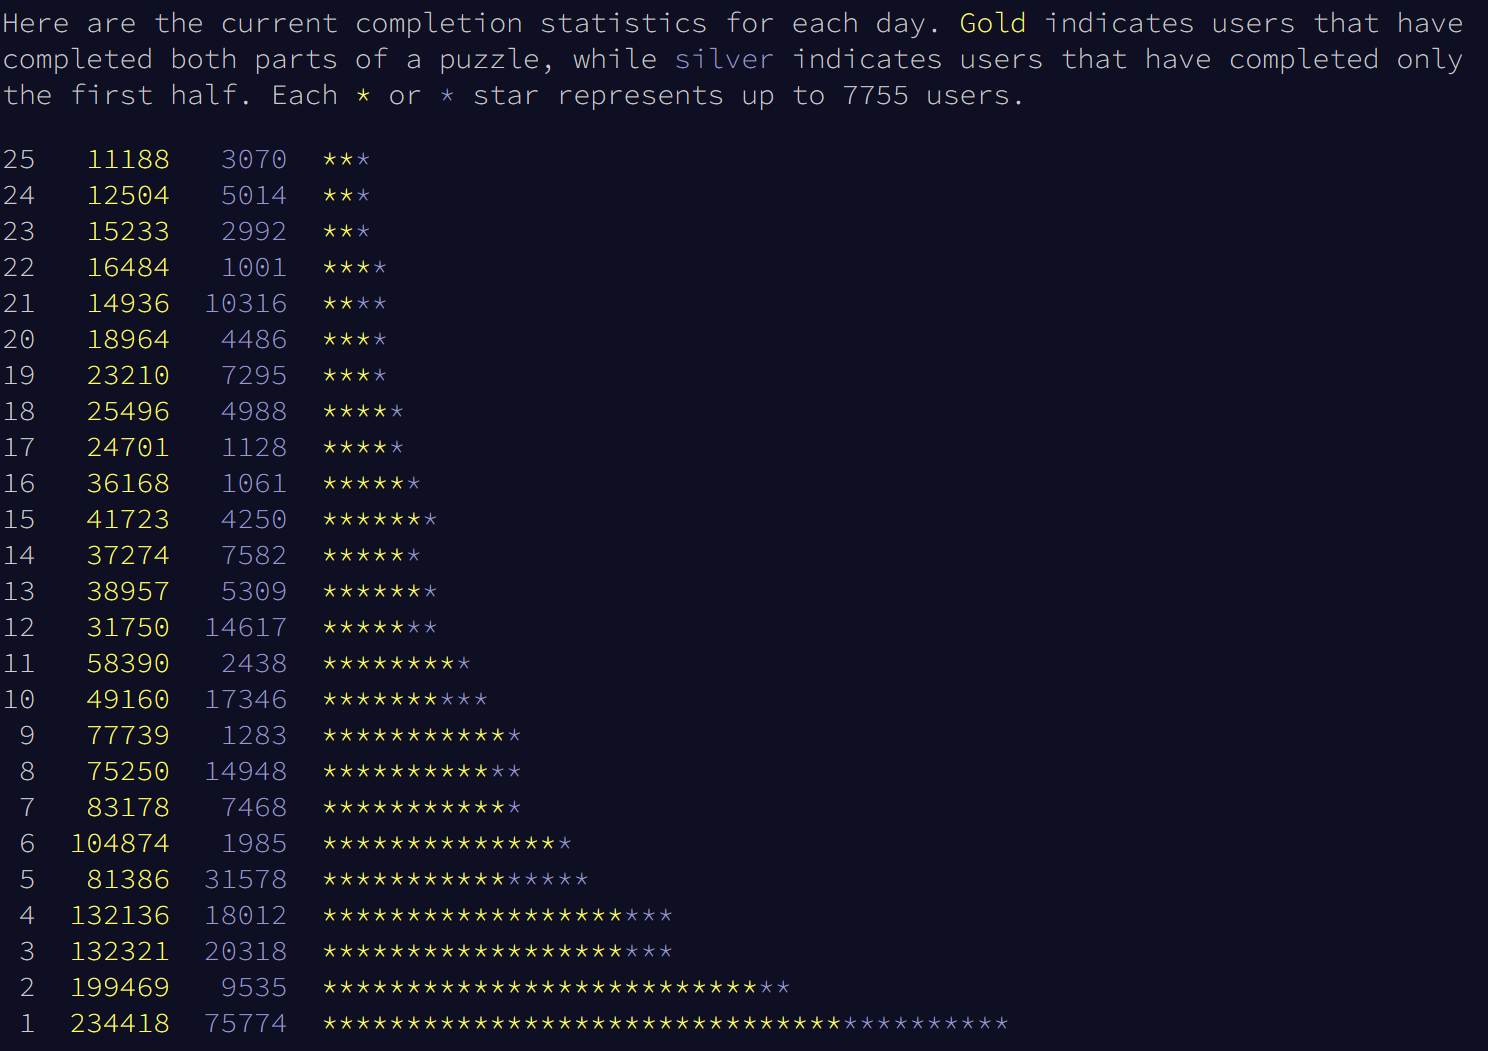
\includegraphics[width=\textwidth]{stats}
\end{center}

\httpsURL{adventofcode.com/2023/stats}
\end{frame}


\begin{frame}
\frametitle{Private Leaderboard}

\begin{center}
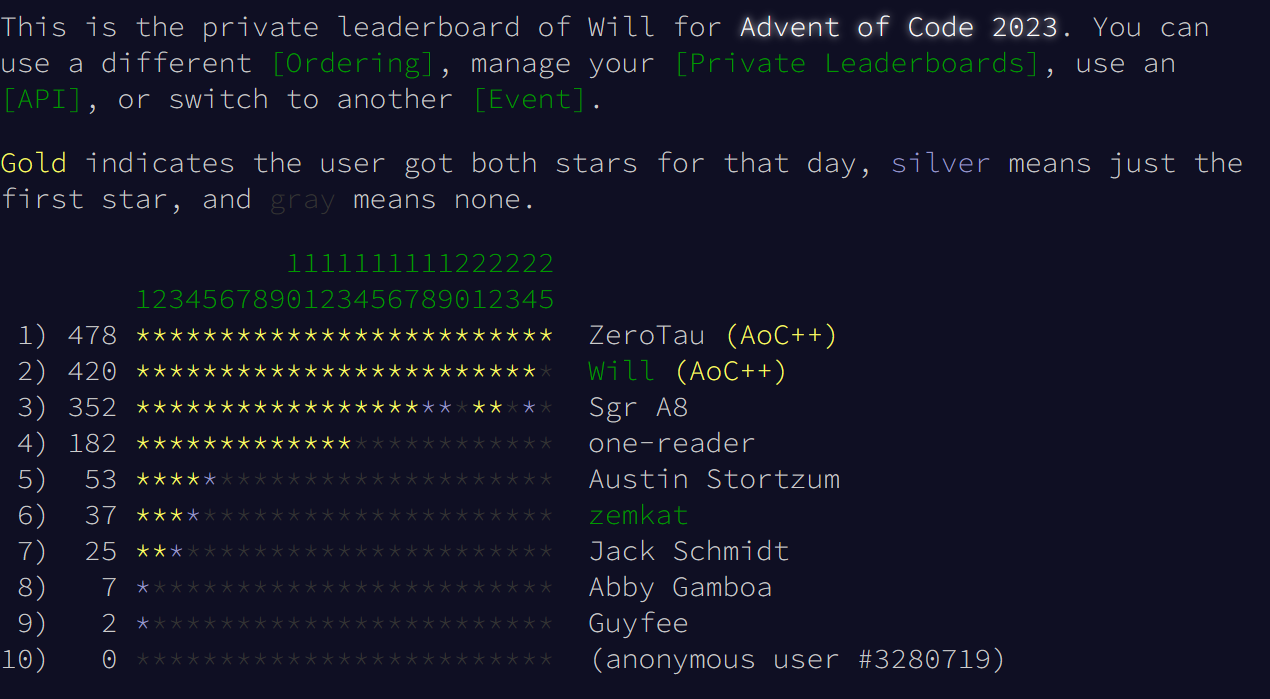
\includegraphics[width=\textwidth]{PrivateLeaderboard}
\end{center}

\end{frame}

\begin{frame}
\frametitle{Global Leaderboard}

\begin{center}
\includegraphics[width=\textwidth]{leaderboard}
\end{center}

\httpsURL{adventofcode.com/2023/leaderboard}

\end{frame}

\begin{frame}
\frametitle{Why do contests?}

\begin{itemize}
  \setlength\itemsep{1em}
  \item Fun
  \item Learning
  \item Community
  \item Profit?
\end{itemize}

\end{frame}

\begin{frame}
\frametitle{Once you see it...}

\begin{center}
  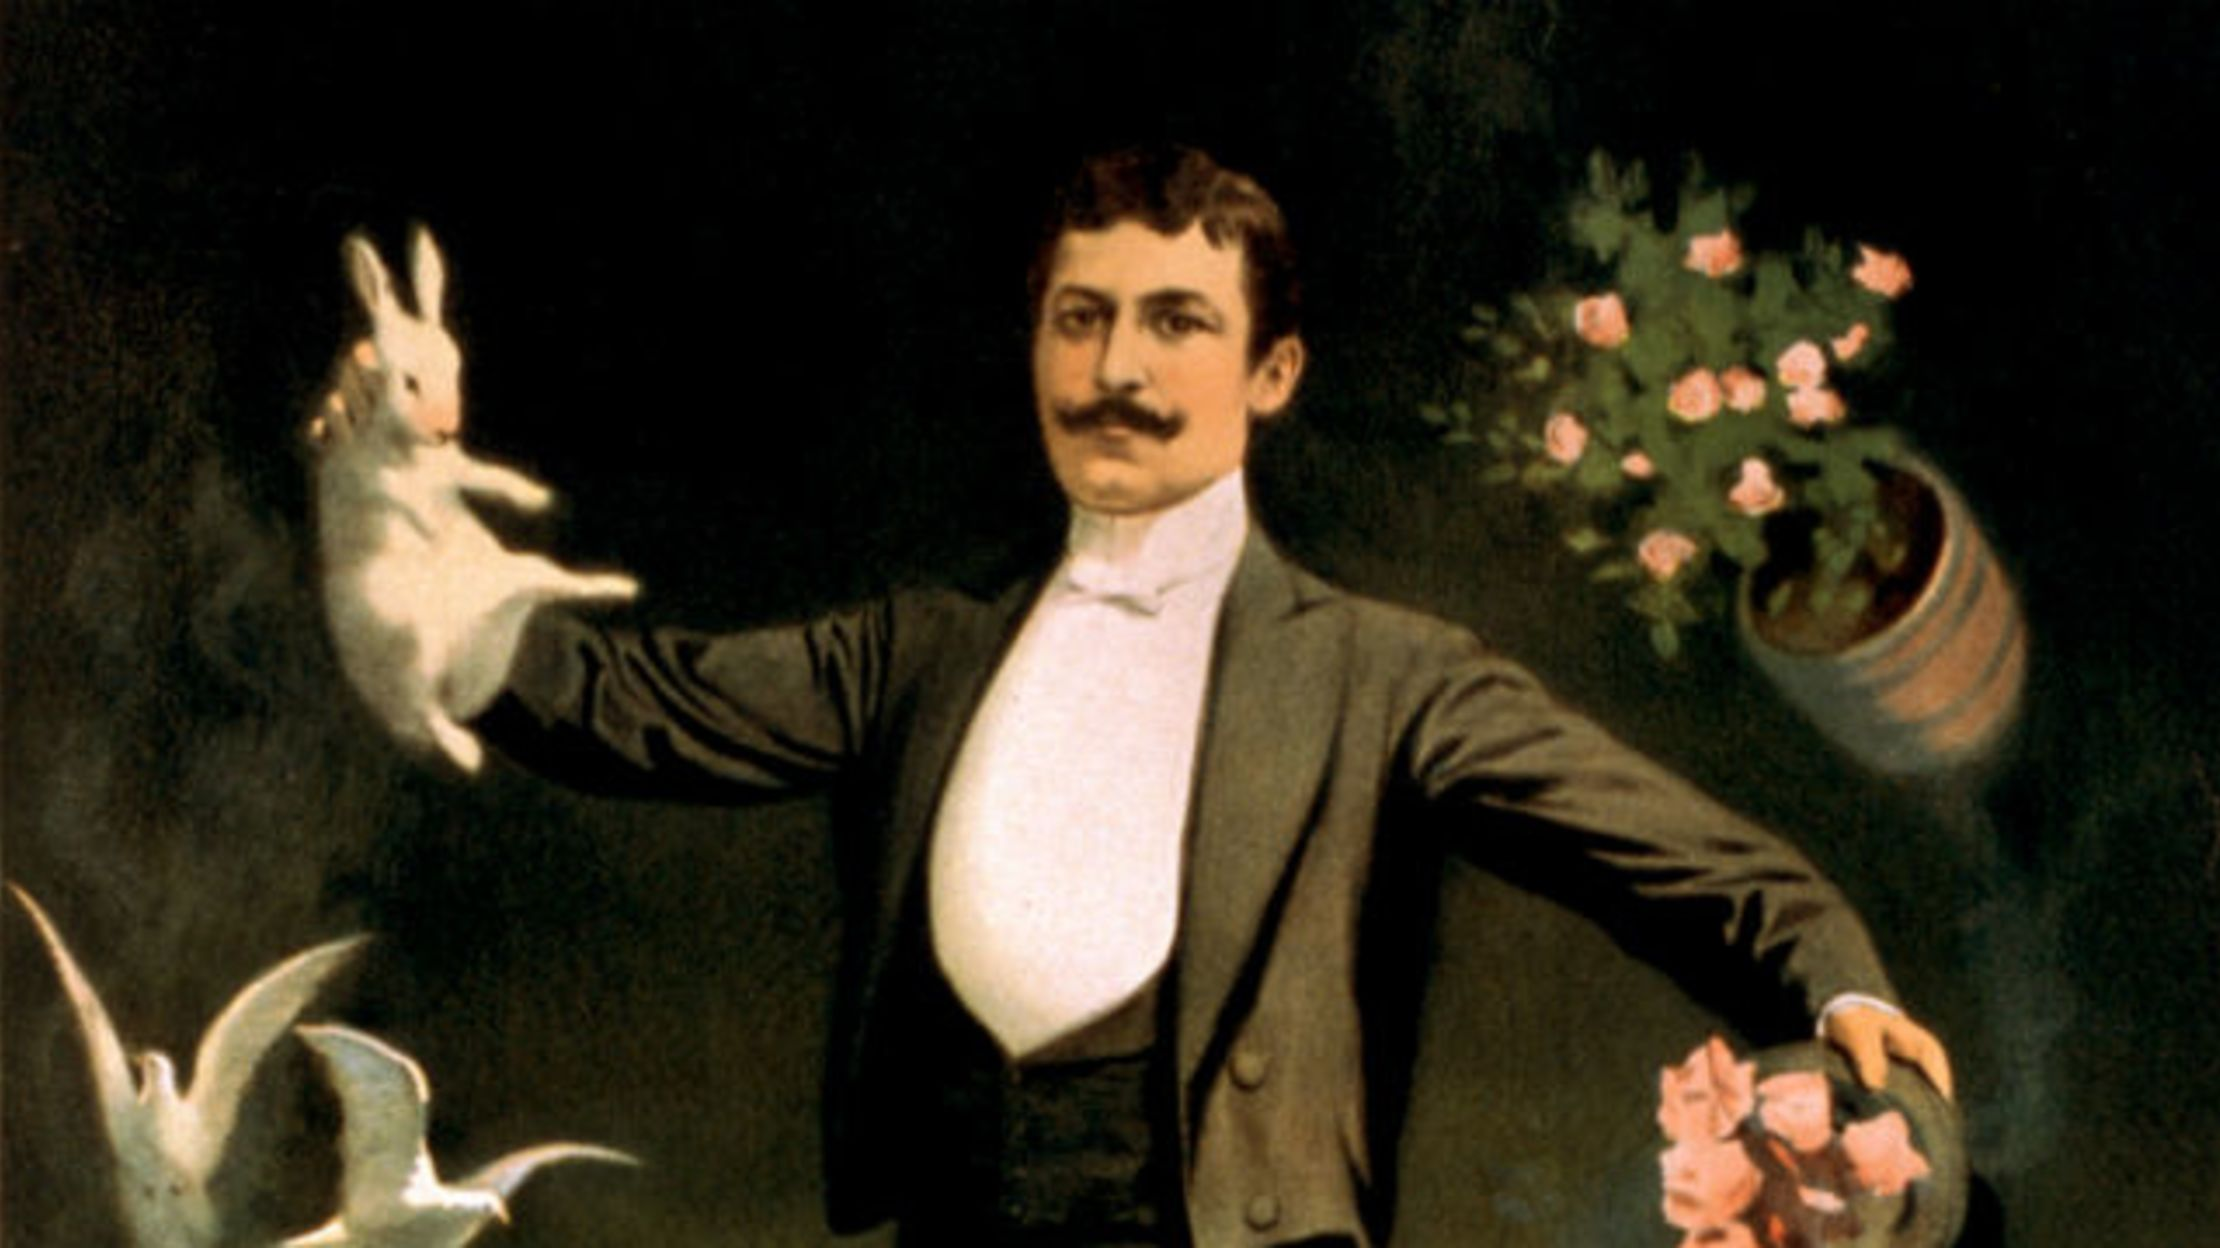
\includegraphics[width=\textwidth]{magician.jpg}
\end{center}

\end{frame}

\begin{frame}
\frametitle{Day 1: Sum of Digits}

This problem asks us to parse lines of input to find the first and last digits contained within.\vfill

Then combine the first digit and the last digit to form a single two-digit number, and sum all such numbers.\vfill

The catch is the digits could be spelled out or written as numbers.
\end{frame}

\begin{frame}[fragile]
\frametitle{Day 1: Example}

\begin{verbatim}
two1nine
eightwothree
abcone2threexyz
xtwone3four
4nineeightseven2
zoneight234
7pqrstsixteen
\end{verbatim}

Yields the sum $29 + 83 + 13 + 24 + 42 + 14 + 76 = 281$.

\end{frame}

\begin{frame}
\frametitle{Day 1: Possible Approaches}

\begin{itemize}
    \item Use a regular expression
    \item Build our own parser
    \item Use tools like sed or awk
    \item Use a parser generator like ANTLR
\end{itemize}\vfill

Note the input is small (around 22KB).\vfill

While we can find the digits with only one pass over the input. Even if we
take multiple passes, we can still solve the problem quickly for input
this small.
\end{frame}

\begin{frame}
\frametitle{Day 1: Possible Approaches}

\begin{itemize}
    \item Use a regular expression
    \item Build our own parser
    \item Use tools like sed or awk
    \item Use a parser generator like ANTLR
\end{itemize}\vfill

Note the input is small (around 22KB).\vfill

While we can find the digits with only one pass over the input. Even if we
take multiple passes, we can still solve the problem quickly for input
this small.
\end{frame}

\begin{frame}
\frametitle{Day 1: Solutions}

\begin{itemize}
    \item Python
    \item Bash pipeline
    \item Circuit
\end{itemize}

\end{frame}

\begin{frame}
\frametitle{Day 16: Light Propagation}
This problem asks us to illuminate as many cells of a room as possible by
shining a light from any cell on an outer edge.\vspace{3em}

This is complicated by the fact that there are mirrors and beam splitters
in the room.
\end{frame}

\begin{frame}[fragile]
\frametitle{Day 16: Rules}
If the beam encounters empty space (\verb!.!), it continues in the same direction.\vfill

If the beam encounters a mirror (\verb!/! or \verb!\!), the beam is reflected 90 degrees depending on the angle of the mirror.\vfill

If the beam encounters the pointy end of a splitter (\verb!|! or \verb!-!), the beam passes as if the splitter were empty space.\vfill

If the beam encounters the flat side of a splitter (\verb!|! or \verb!-!), the beam is split into two beams going in each of the two directions the splitter's pointy ends are pointing.\vfill

Beams do not interact with other beams
\end{frame}

\begin{frame}[fragile]
\frametitle{Day 16: Example}

\begin{center}
\begin{minipage}{0.45\textwidth}
\begin{center}
\begin{verbatim}
.|...\....
|.-.\.....
.....|-...
........|.
..........
.........\
..../.\\..
.-.-/..|..
.|....-|.\
..//.|....
\end{verbatim}
\end{center}
\end{minipage}
\begin{minipage}{0.45\textwidth}
\begin{center}
\begin{verbatim}
>|<<<\....
|v-.\^....
.v...|->>>
.v...v^.|.
.v...v^...
.v...v^..\
.v../2\\..
<->-/vv|..
.|<<<2-|.\
.v//.|.v..
\end{verbatim}
\end{center}
\end{minipage}
\end{center}
\vfill

In this example, 46 cells are {\it illuminated} when light shines in from the left in the top left cell.
\end{frame}

\begin{frame}
\frametitle{Day 16: Instance Size}

Our problem input is a room with 110 rows and 110 columns.\vfill

So there are 12100 cells.\vfill

Our instance has 1191 objects in the room.\vfill

What are the challenges of this problem?\vfill

Let's look at a solution.
\end{frame}

\begin{frame}
\frametitle{Day 18: Lavaduct Lagoon}

    \begin{center}
        Given instructions consisting of direction and distance to dig out the edge of a pit, what will the resulting area of the pit be?
    \end{center}

\end{frame}

\begin{frame}[fragile]
\frametitle{Day 18: Example}
    
    \begin{center}
        \begin{minipage}{0.3\textwidth}
        \begin{center}
        \begin{verbatim}
R 6
D 5
L 2
D 2
R 2
D 2
L 5
U 2
L 1
U 2
R 2
U 3
L 2
U 2
        \end{verbatim}
        \end{center}
        \end{minipage}
        \begin{minipage}{0.3\textwidth}
        \begin{center}
        \begin{verbatim}
#######
#.....#
###...#
..#...#
..#...#
###.###
#...#..
##..###
.#....#
.######
        \end{verbatim}
        \end{center}
        \end{minipage}
        \begin{minipage}{0.3\textwidth}
            \begin{center}
            \begin{verbatim}
#######
#######
#######
..#####
..#####
#######
#####..
#######
.######
.######
            \end{verbatim}
            \end{center}
            \end{minipage}
    \end{center}
    \vfill

\end{frame}

\begin{frame}
\frametitle{Day 18: Bigmode}

Finding the area of these small shapes isn't too bad.\vfill

Could use a left-to-right scan, flood fill, whatever, and computationally be alright. But what if it was much bigger?\vfill

Part 2: Oops, instead of numbers from 2 to 12, we meant to give you a 5 digit hexadecimal number.\vfill

Our answer has now gone from a magnitude of 1e4 to 1e14.\vfill

\end{frame}

\begin{frame}
\frametitle{Day 18: Thinking with Shapes}

Storing and computing is now out of the question.*\vfill

New approach: thinking. What is it that we need the area of?\vfill

How can we get the area of that?\vfill

\end{frame}

\begin{frame}[fragile]
\frametitle{Day 18: Shoelace, Gauss, Surveyor's, etc.}

\begin{center}
$A = \frac{1}{2}\sum_{i=1}^{n}(y_i + y_{i+1})(x_i - x_{i+1})$\vfill
\end{center}

\begin{center}

\begin{minipage}{0.3\textwidth}
\begin{center}
\begin{verbatim}
A-----B
|.....|
N-M...|
..|...|
..|...|
K-L.D-C
|...|..
JI..E-F
.|....|
.H----G
\end{verbatim}
\end{center}
\end{minipage}
\begin{minipage}{0.3\textwidth}
\begin{center}
$(y_{A} + y_{B})(x_{A} - x_{B})$
$(y_{B} + y_{C})(x_{B} - x_{C})$
$(y_{C} + y_{D})(x_{C} - x_{D})$
$(y_{D} + y_{E})(x_{D} - x_{E})$
...
$(y_{N} + y_{A})(x_{N} - x_{A})$
\end{center}
\end{minipage}

\end{center}
\vfill

\end{frame}

\begin{frame}
\frametitle{Day 18: Pick's Theorem}

Our area calculation is still a smidge short.\vfill

If we consider ourselves to be digging out a cube block of dirt, we're standing in the center of the block and therefore not counting all of it when digging.\vfill

Enter Pick's Theorem: $A = i + \frac{b}{2} - 1$

\end{frame}

\begin{frame}
\frametitle{Day 18: Visualization}

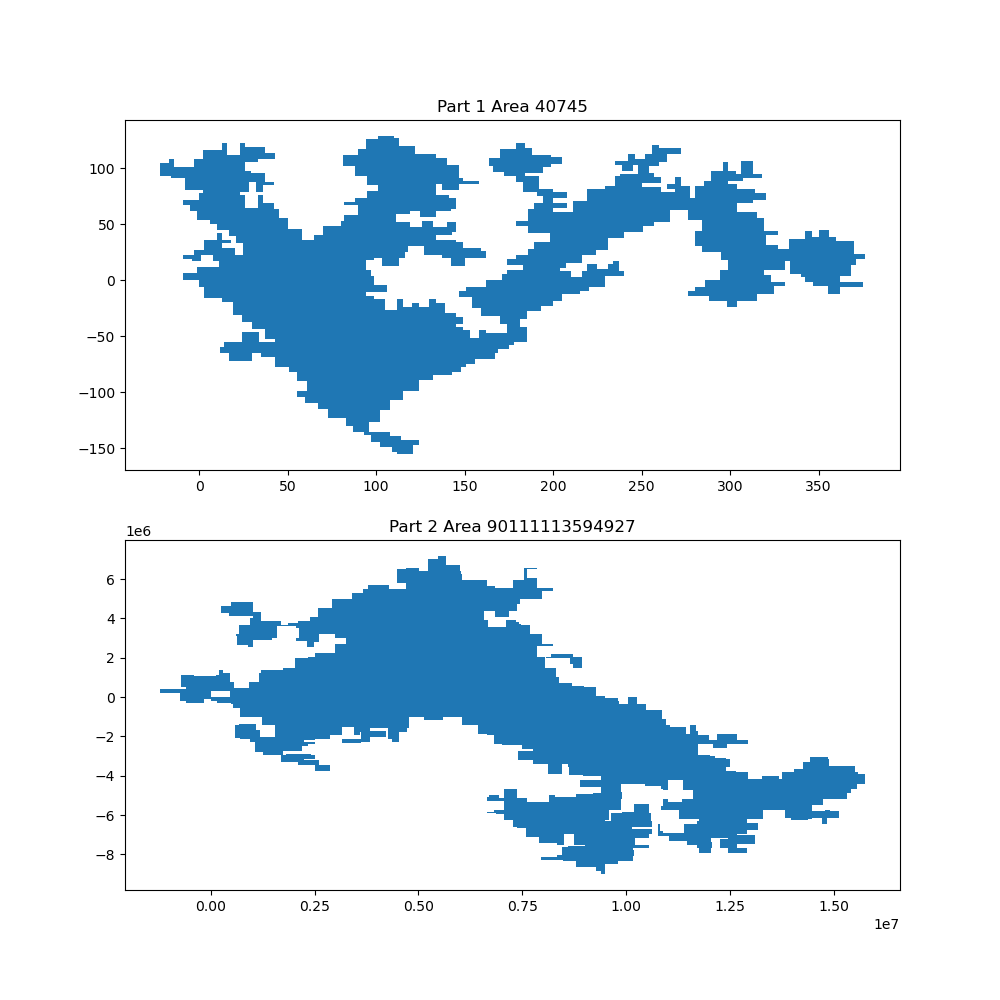
\includegraphics[height=\textheight]{Day18}

\end{frame}
\begin{frame}
\frametitle{Day 20: Pulse Propagation}

You have a collection of modules that can send and receive high or low pulses connected together. There are three main types:
\begin{itemize}
    \item Flip-flop modules $(\%)$, when receiving a low pulse, flip their internal state between sending a high pulse or a low pulse, defaulting to high.
    \item Conjunction modules $(\&)$ remember the most recent pulses from each input, defaulting their memory to low - if all pulses in memory are high, it sends a low pulse, else high.
    \item There is a button/broadcast module that sends a low pulse to all of its destination modules.
\end{itemize}\vfill

Pulses are processed in the order they are sent.

\end{frame}

\begin{frame}
\frametitle{Day 20: Button}

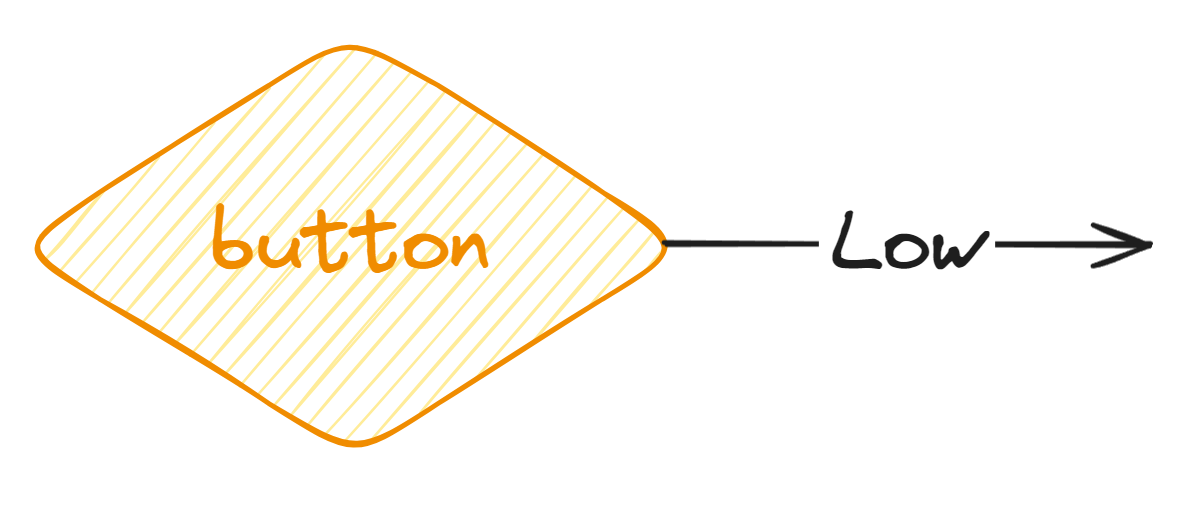
\includegraphics[width=\textwidth]{Day20Button}

\end{frame}

\begin{frame}
\frametitle{Day 20: Flip Flop}

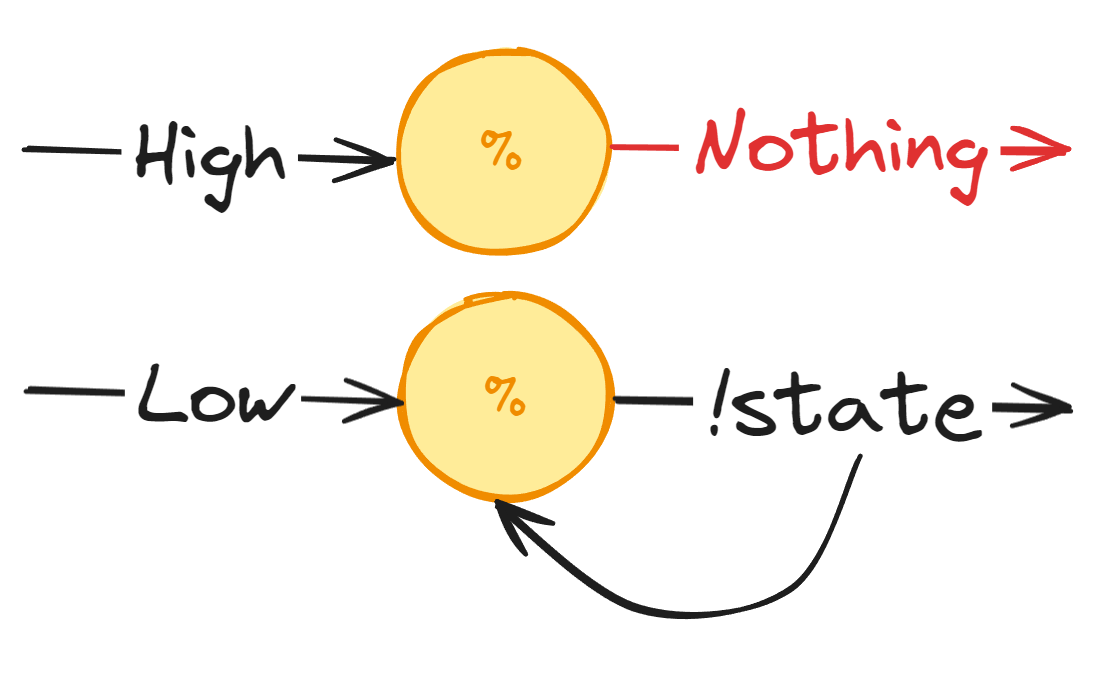
\includegraphics[width=\textwidth]{Day20FlipFlop}

\end{frame}


\begin{frame}
\frametitle{Day 20: Conjunction}

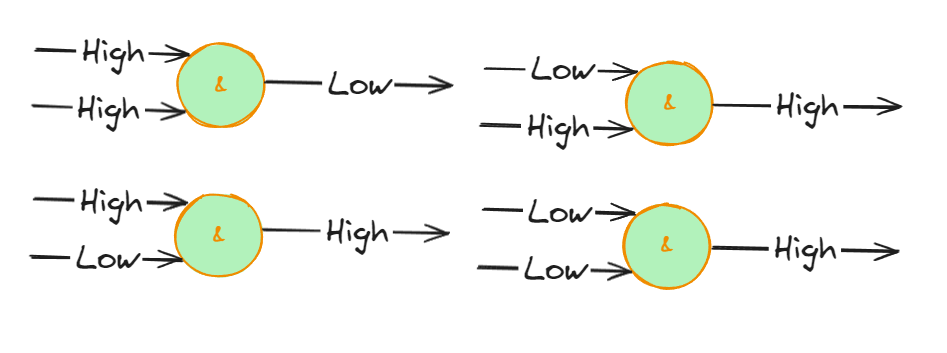
\includegraphics[width=\textwidth]{Day20Conjunction}

\end{frame}

\begin{frame}[fragile]
\frametitle{Day 20: Example}

\begin{center}
\begin{minipage}{0.45\textwidth}
\begin{center}
\begin{verbatim}
btn -> a, b, c
%a -> b
%b -> c
%c -> inv
&inv -> a        
\end{verbatim}
\end{center}
\end{minipage}
\begin{minipage}{0.45\textwidth}
\begin{center}
\begin{verbatim}
btn -low-> a
btn -low-> b
btn -low-> c
a -high-> b
b -high-> c
c -high-> inv
inv -low-> a
a -low-> b
b -low-> c
c -low-> inv
inv -high-> a        
\end{verbatim}
\end{center}
\end{minipage}
\end{center}

\end{frame}

\begin{frame}[fragile]
\frametitle{Day 20: Example Cont.}

\begin{center}
\begin{verbatim}
                   a:1, b:1, c:1, inv:[c:0]
btn -low-> a       a:0, b:1, c:1, inv:[c:0]
btn -low-> b       a:0, b:0, c:1, inv:[c:0]
btn -low-> c       a:0, b:0, c:0, inv:[c:0]
a -high-> b        a:0, b:0, c:0, inv:[c:0]
b -high-> c        a:0, b:0, c:0, inv:[c:0]
c -high-> inv      a:0, b:0, c:0, inv:[c:1]
inv -low-> a       a:1, b:0, c:0, inv:[c:1]
a -low-> b         a:1, b:1, c:0, inv:[c:1]
b -low-> c         a:1, b:1, c:1, inv:[c:1]
c -low-> inv       a:1, b:1, c:1, inv:[c:0]
inv -high-> a      a:1, b:1, c:1, inv:[c:0]
\end{verbatim}
\end{center}

\end{frame}

\begin{frame}
\frametitle{Day 20: Part 1}

After 1,000 button presses, how many pulses were sent?\vfill

Simulation go brrr

\end{frame}

\begin{frame}
\frametitle{Day 20: Part 2}

We want to know how many button presses are required to send a single low pulse to module rx.\vfill

Simulation go brrr... for a long time. A bit over 270,000 times longer. Clearly, computation is not the way to go.\vfill

\end{frame}

\begin{frame}
\frametitle{Day 20: Graph (Unified)}

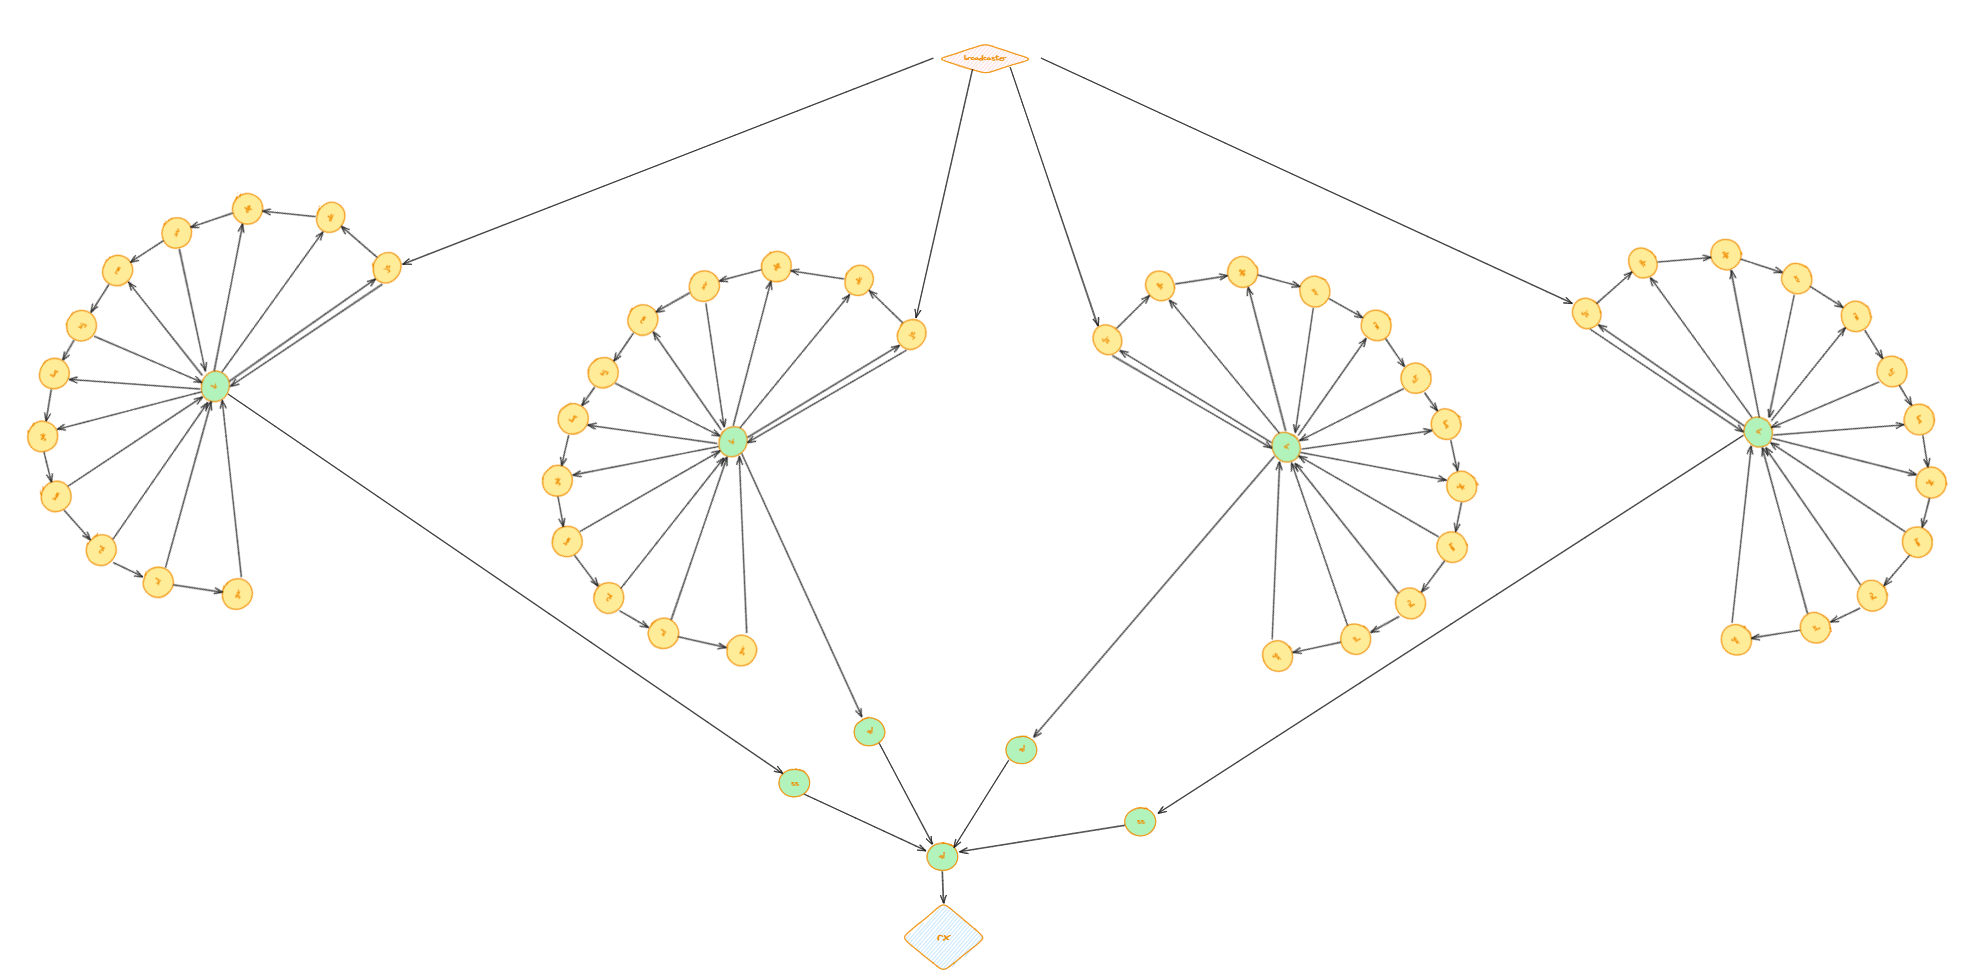
\includegraphics[width=\textwidth]{Day20GraphUnified}

\end{frame}

\begin{frame}
\frametitle{Day 20: Graph (Separate)}

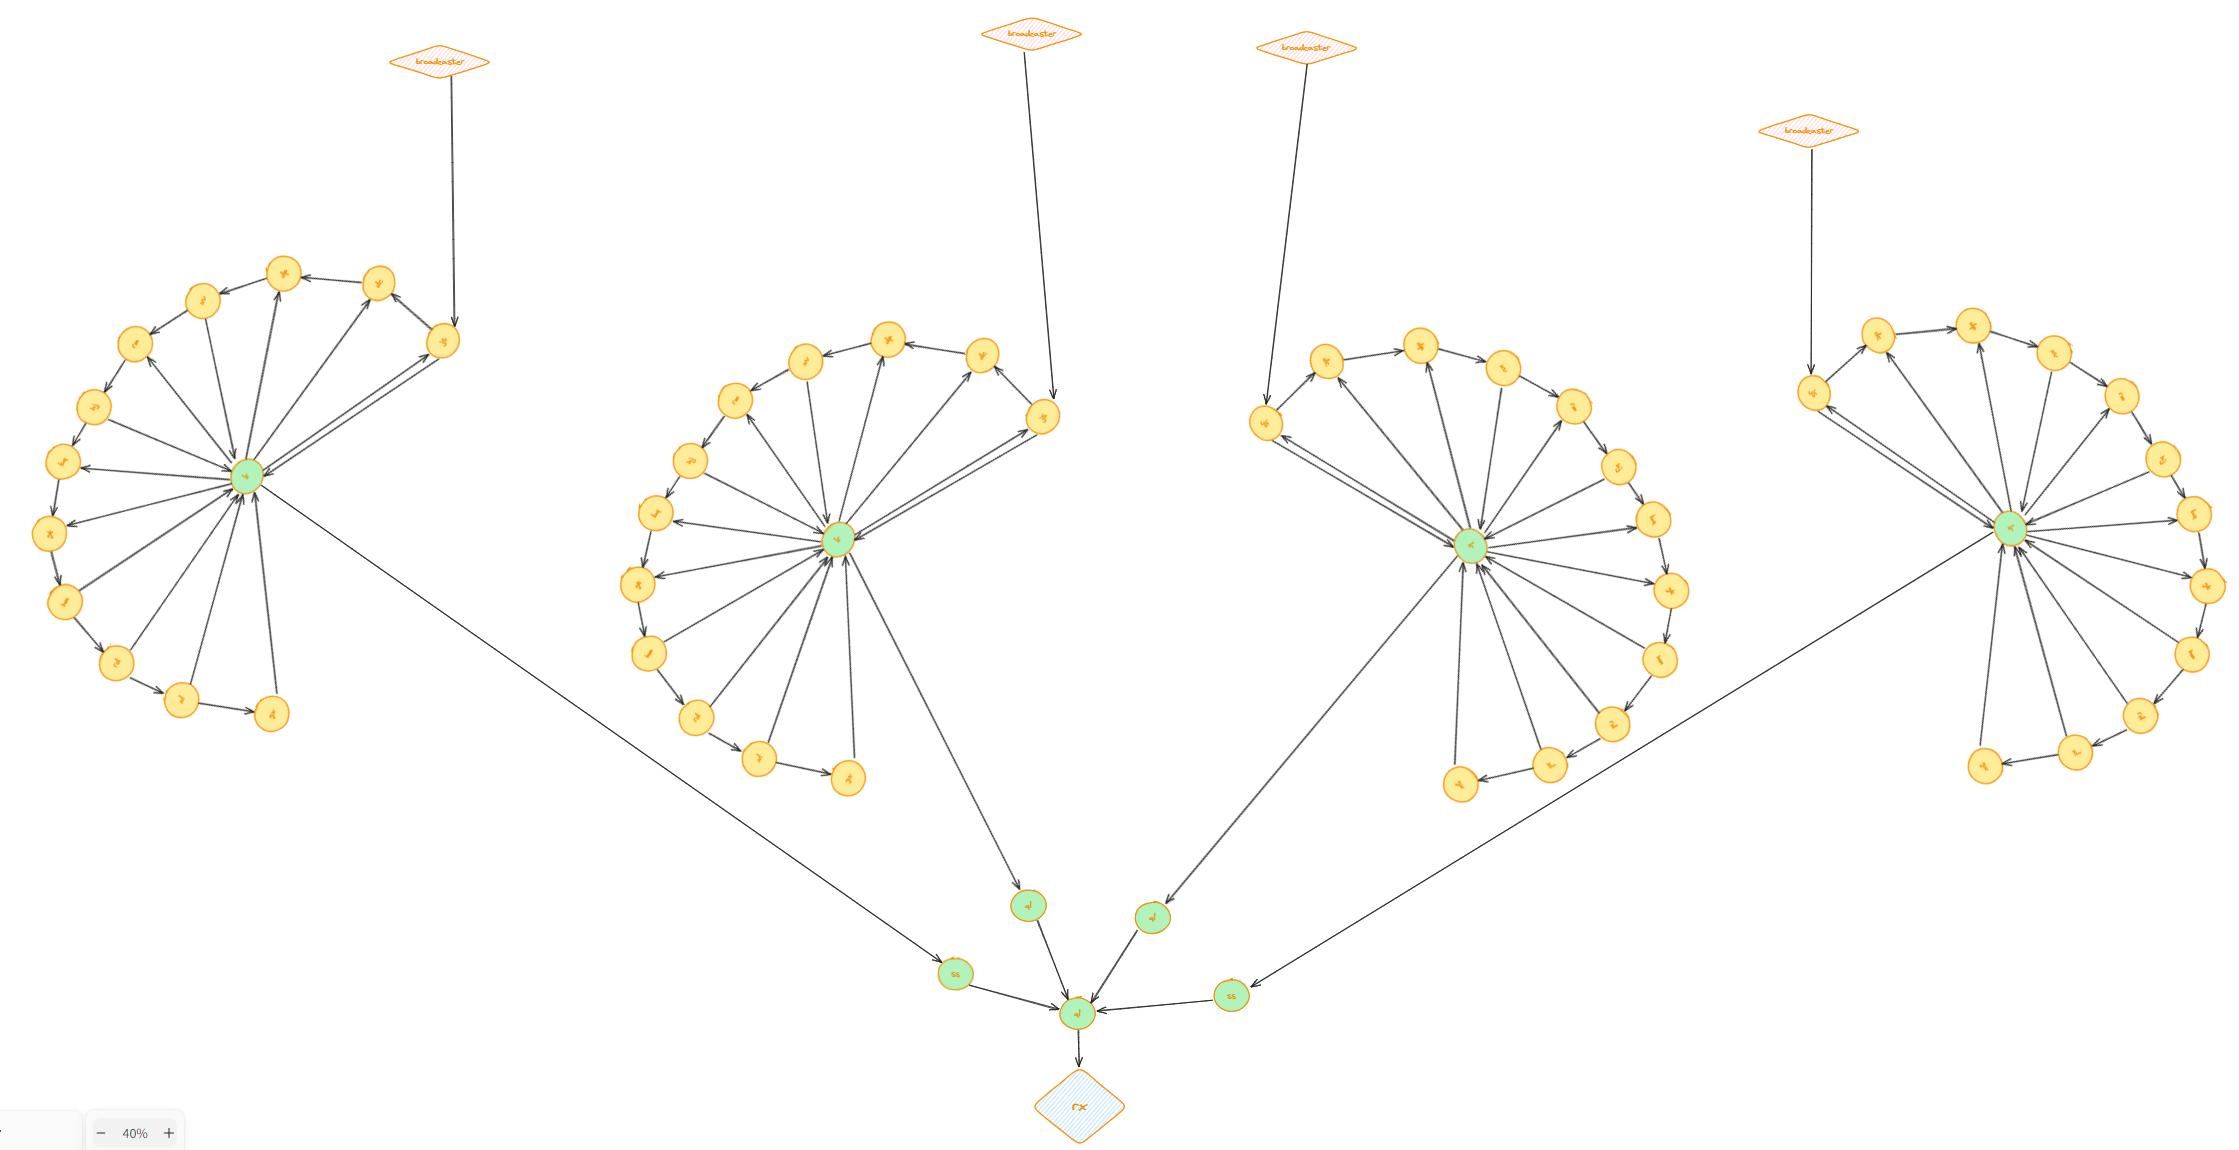
\includegraphics[width=\textwidth]{Day20GraphSeparate}

\end{frame}

\begin{frame}
\frametitle{Day 20: Graph (Black Box)}

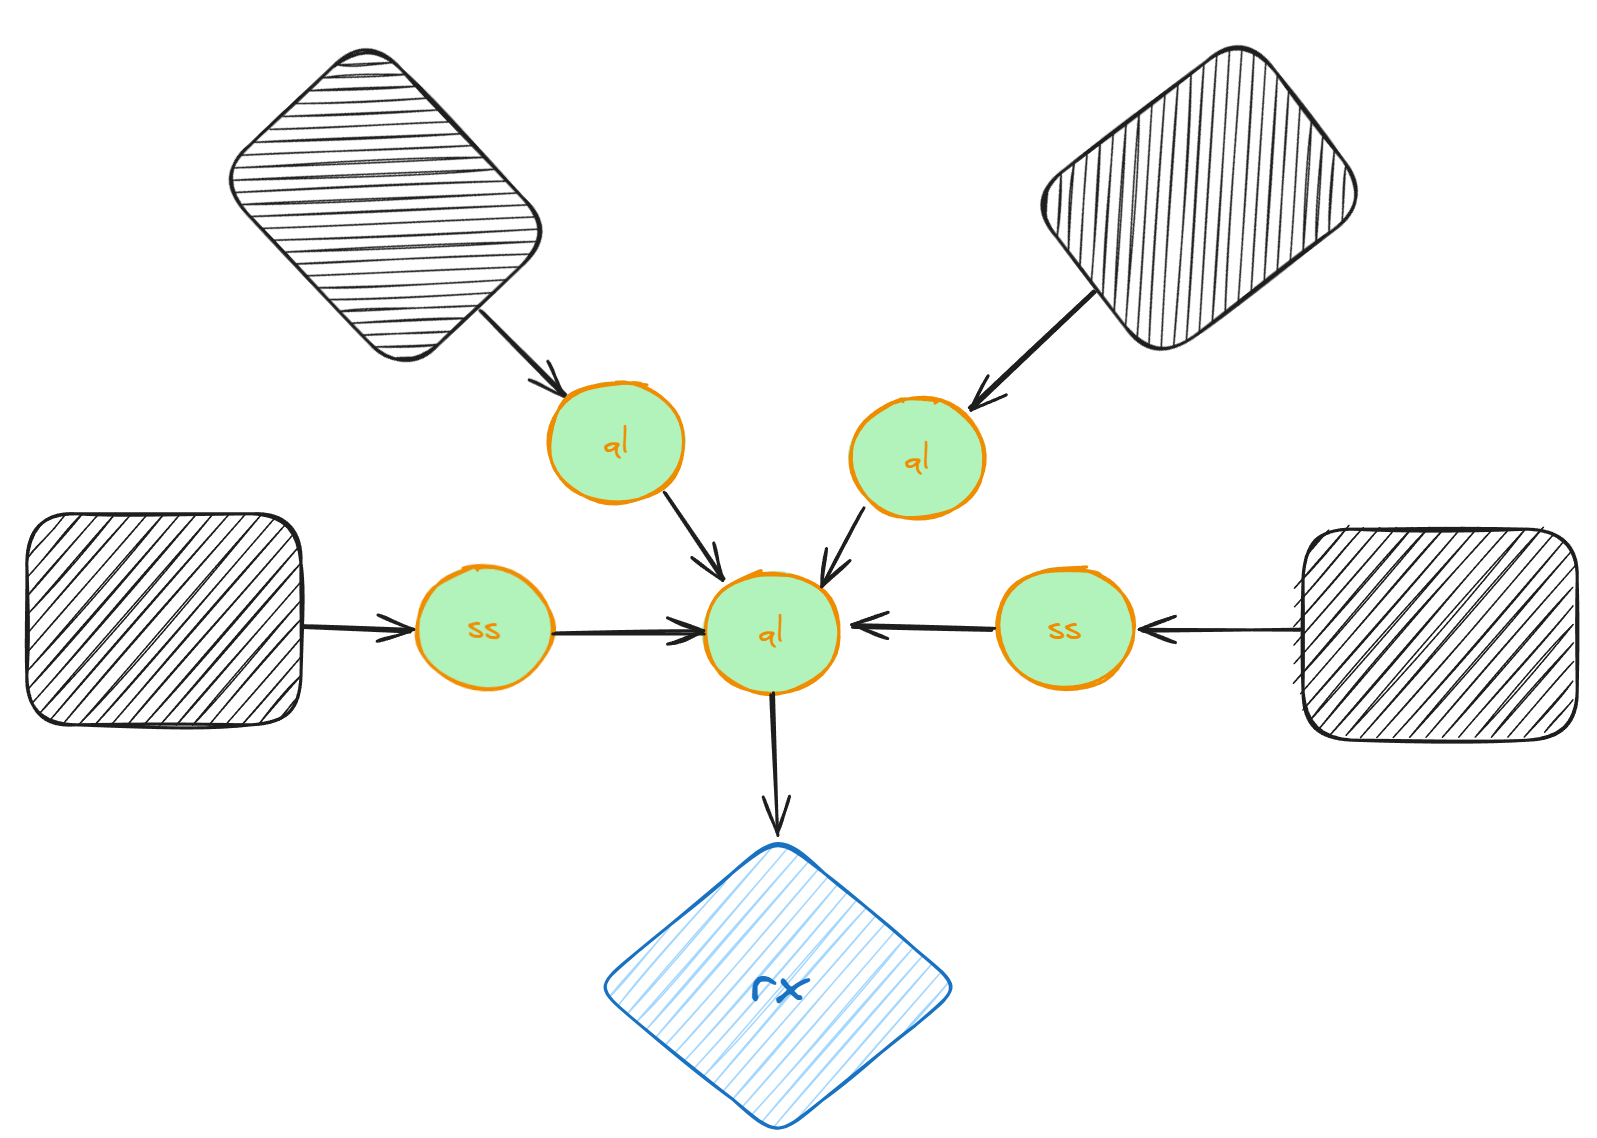
\includegraphics[width=\textwidth]{Day20BlackBox}

\end{frame}

\begin{frame}
\frametitle{Day 20: Break It Down}

Module rx only receives input from dr.\linebreak
Module dr only receives input from qt, qb, ng, mp.\linebreak
Modules qt, qb, ng, mp each receive input from a unique subgraph.\vfill

Each subgraph can be "solved" independently.

\end{frame}
\begin{frame}
\frametitle{Day 21: Infinite Maze}

For the first part of the problem we are given a maze of open and
impassable cells, and asked how many locations can be reached in exactly
a given number of steps.\vfill

Note we are allowed to return locations we have already visited.\vfill

The maze has 131 rows and 131 columns. So this can be brute forced.
\end{frame}

\begin{frame}
\frametitle{Day 21: Infinite Maze}

For the second part of the problem, the maze we were given is tiled in each direction to form
an infinite maze. \vfill

We are asked to find the number of locations that can be reached in exactly 26,501,365 steps.\vfill

This will take a long time to brute force.

\end{frame}

\begin{frame}
\frametitle{Day 21: Instance}

Let's look at our instance of the problem. \vfill

Note the structure of our maze has a lot of regularity.\vfill

Also, while the full number of steps is too large to brute force,
we can solve many smaller instances.\vfill

Here is the data in Mathematica.
\end{frame}

\begin{frame}
\frametitle{Day 24: Never Tell Me The Odds}

You're surrounded by hailstones, each with a given position and velocity\vfill
PX, PY, PZ @ VX, VY, VZ\vfill

Part 1: Looking forward in time, how many of the hailstones' paths will intersect within a test area?\vfill

Make it simpler:
\begin{itemize}
    \item Forward in time: t $>$ 0
    \item Paths will intersect: hailstones themselves don't have to collide
    \item Within a test area: specific bounds
    \item Also, ignore the Z axis.
\end{itemize}

\end{frame}

\begin{frame}
\frametitle{Day 24: Never Tell Me The Odds}

If we know a starting point and our change, what are we actually working with?\vfill % Lines

How easy is it to see if lines intersect?\vfill % Very easy

\end{frame}

\begin{frame}
\frametitle{Day 24: Never Tell Me The Odds, Continued}
    
Although the paths cross, no hailstones will actually collide on their current course. If you throw a rock just right, you can hit every hailstone! \vfill
Thanks to magic, the rock can start at any integer position and velocity. \vfill
Where and how quickly to throw the rock? \vfill
    
\end{frame}

\begin{frame}
\frametitle{Day 24: Never Tell Me The Odds, Continued}
    
Now we don't know PX, PY, PZ, VX, VY, or VZ for our rock\vfill

We do know that at some time $T$, our rock will collide with a hailstone at position $X, Y, Z$\vfill

No guarantee that $T_1$ = 1, $T_2$ = 2, etc., so $T$ is unknown.\vfill
    
\end{frame}

\begin{frame}
\frametitle{Day 24: Putting Together the Unknowns}
    
So we have 7 unknowns: PX, PY, PZ, VX, VY, VZ, and T.\vfill

What do we know?\vfill

At $T_1$, $X_{rock}, Y_{rock}, Z_{rock} = X_{hail_1}, Y_{hail_1}, Z_{hail_1}$\vfill

$Pos_T = Pos_{Start} + Velocity(T)$\linebreak
$X_{rock} = PX + VX(T)$\linebreak
$X_{hail_1} = PX_{hail_1} + VX_{hail_1}(T)$\vfill

Now we're adding in equations with known variables.

\end{frame}
\begin{frame}[fragile]
\begin{center}

\begin{tikzpicture}
  \fill[color=blue!10] (-5,-2.5) rectangle (5,2.5);
  \path (0,0) node {{\Huge \color{blue} Questions?}};
\end{tikzpicture}
\end{center}
\vfill
This talk available at \httpsURL{github.com/ZeroTau/AoC2023Talk}
\end{frame}

\begin{frame}\frametitle{}

\begin{center}

\begin{tikzpicture}
  \fill[color=green!60!black!25] (-5,-2.5) rectangle (5,2.5);
  \path (0,0) node {{\Huge \color{blue!75!black!85} Thank You!}};
\end{tikzpicture}
\end{center}
\end{frame}


\end{document}
